% Nitime talk

\documentclass{beamer}

\usepackage{ulem}
\usepackage{listings,bera}

\usetheme{PaloAlto}
\beamertemplatenavigationsymbolsempty

\definecolor{fore}{RGB}{0,20,30}
\definecolor{back}{RGB}{255,255,255}
\definecolor{title}{RGB}{255,255,255}


\setbeamercolor{titlelike}{fg=title}
\setbeamercolor{normal text}{fg=fore,bg=back}
\definecolor{keywords}{RGB}{255,0,90}
\definecolor{comments}{RGB}{60,179,113}
\definecolor{strings}{RGB}{120,120,0}

\lstset{language=Python,
keywordstyle=\color{keywords},
commentstyle=\color{comments}\emph,
stringstyle=\color{strings}}

\title[nitime]{\tt{nitime}}
\subtitle
{{Time-series analysis for neuroscience data in Python}}

\author[Ariel Rokem] % (optional, use only with lots of authors)
{Ariel Rokem}
\date{August 31st, 2011}
\institute[Stanford University]
{Stanford University}

\pgfdeclareimage[height=1.5cm]{ucb-logo}{figures/ucb_logo}
% put nipy logo in bottom left
\pgfdeclareimage[height=1.5cm]{nipper}{figures/nipper}
\setbeamertemplate{sidebar left}{
   \rlap{\hskip0.1cm%
     {\pgfuseimage{ucb-logo}}}
    \vfill%
   \rlap{\hskip0.1cm%
     {\pgfuseimage{nipper}}}%
   \vskip2pt%
   \llap{\usebeamertemplate***{navigation symbols}\hskip0.1cm}%
   \vskip2pt%
}

\begin{document}

%Title page:
\begin{frame}
  \titlepage
\end{frame}

\begin{frame}
\frametitle{Outline}
\begin{itemize}
\pause
\item
Scientific motivation
\pause
\item 
A simple example: coherence
\pause
\item
The \tt{nitime} \sc{software library}
\end{itemize}
\end{frame}

\begin{frame}
\frametitle{Task-specific networks}
  One of the goals of contemporary neuroscience is to delineate task-specific
  networks in the brain
\end{frame}

\begin{frame}
\frametitle{The wiring diagram}
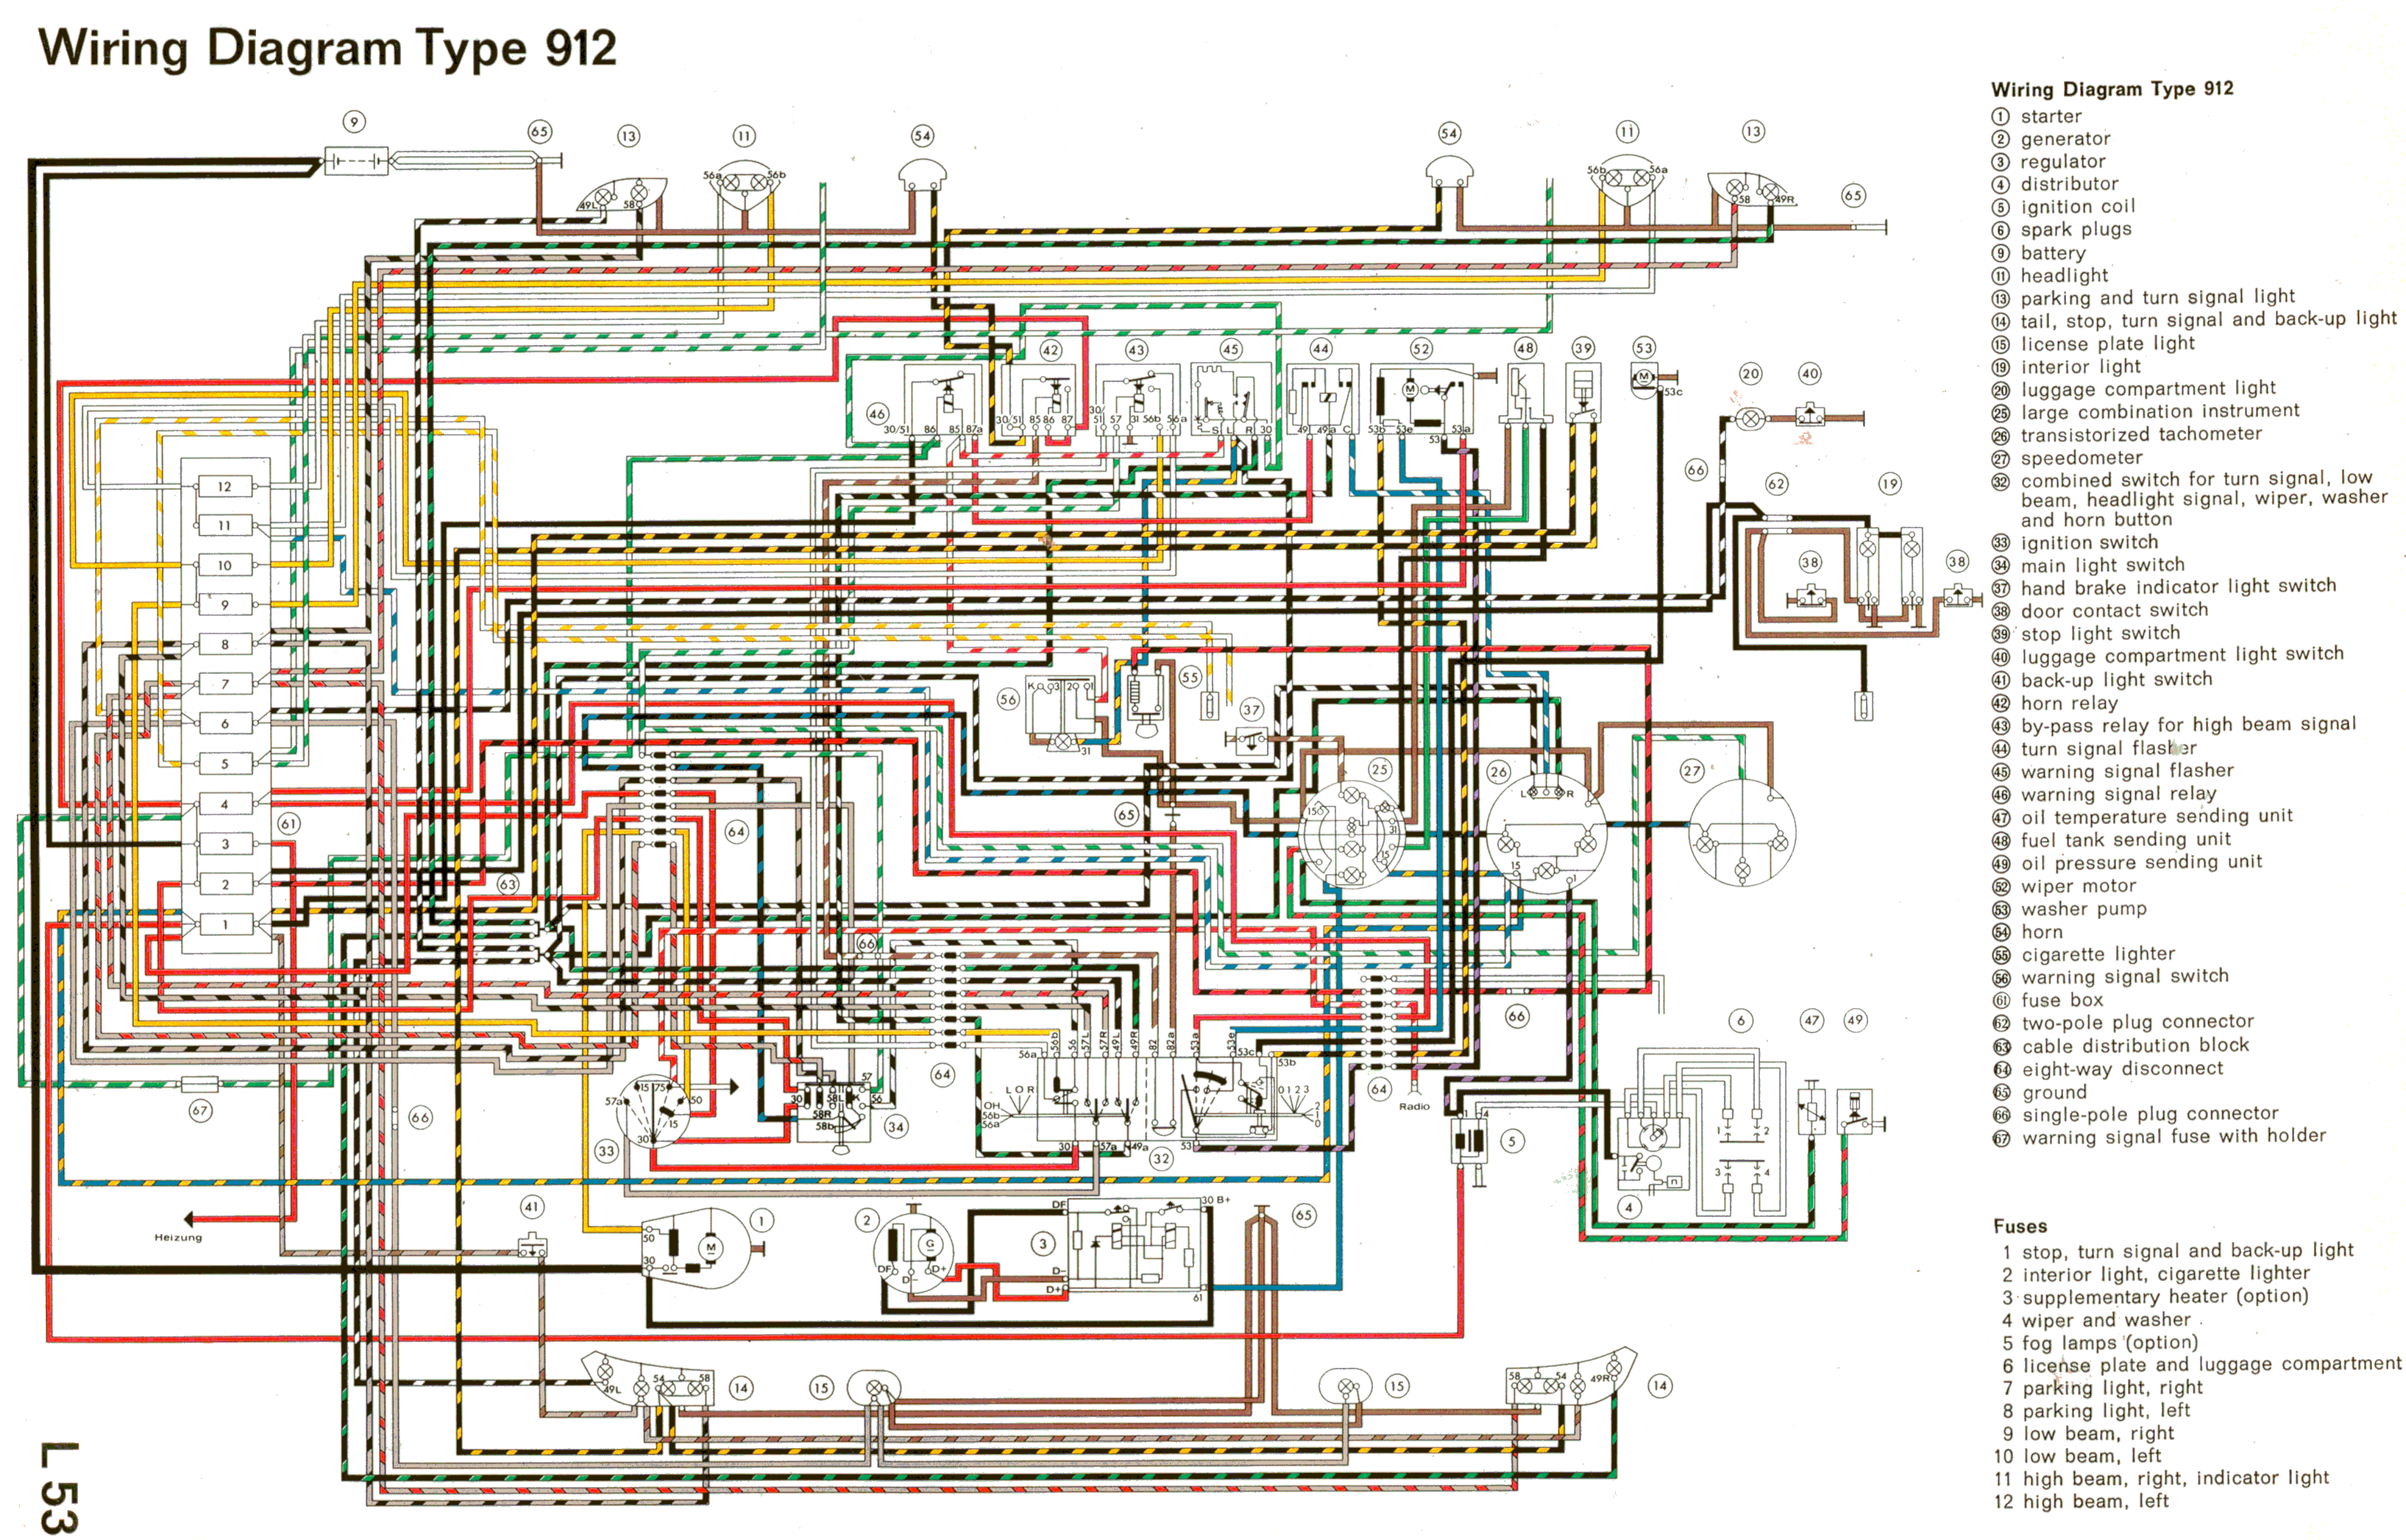
\includegraphics[height=5.7cm]{figures/wiring}
\end{frame}

\begin{frame}
\frametitle{The wiring diagram}
\includegraphics[height=5.7cm]{figures/felleman1}
\\
\hfill
Felleman and Van Essen (1991)
\end{frame}

\begin{frame}
\frametitle{The wiring diagram}
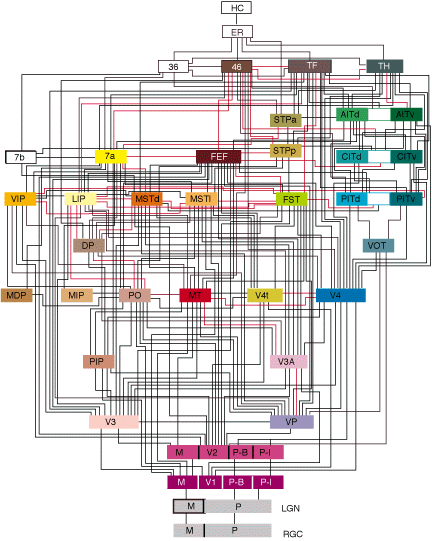
\includegraphics[height=5.7cm]{figures/felleman2}
\\
\hfill
Felleman and Van Essen (1991)
\end{frame}

\begin{frame}
\frametitle{Task-specific networks}
  One of the goals of contemporary neuroscience is to delineate task-specific
  networks in the brain
\end{frame}

\begin{frame}
\frametitle{Time-series in fMRI data}
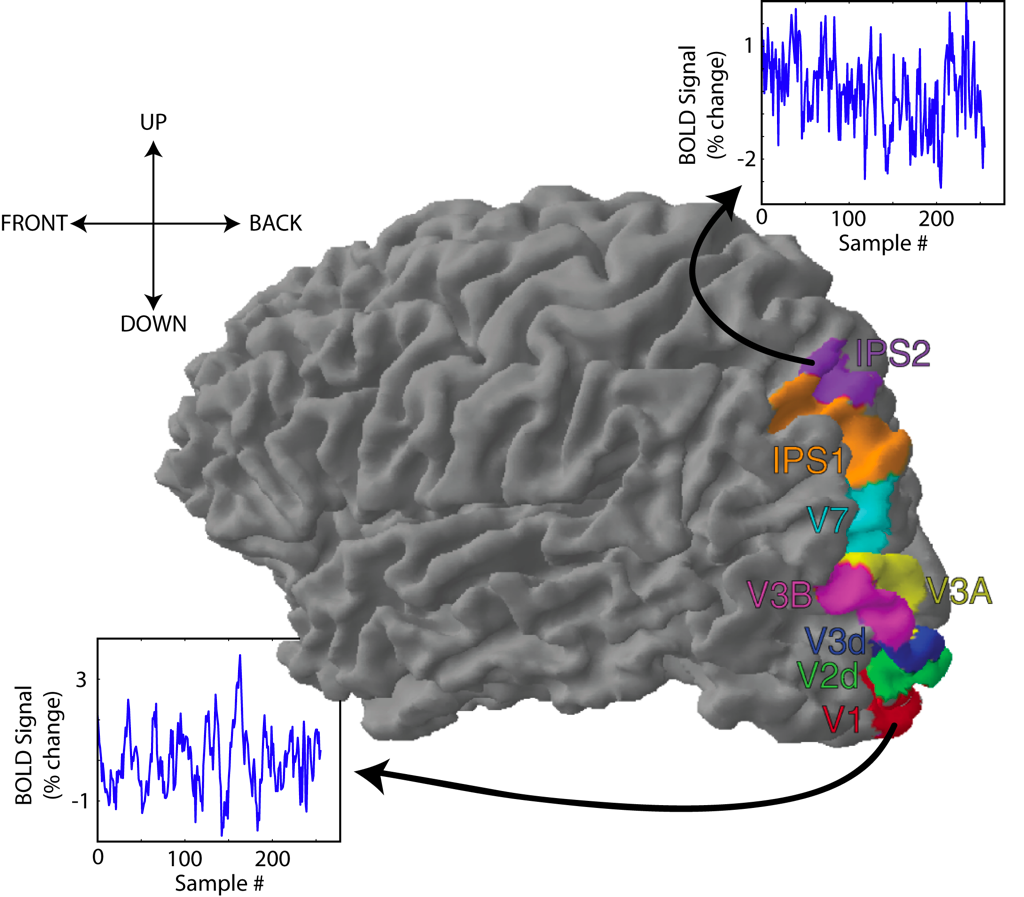
\includegraphics[height=5.7cm]{figures/brain_w_tseries}
\end{frame}

\begin{frame}
\frametitle{Using coherency to study task-related networks}
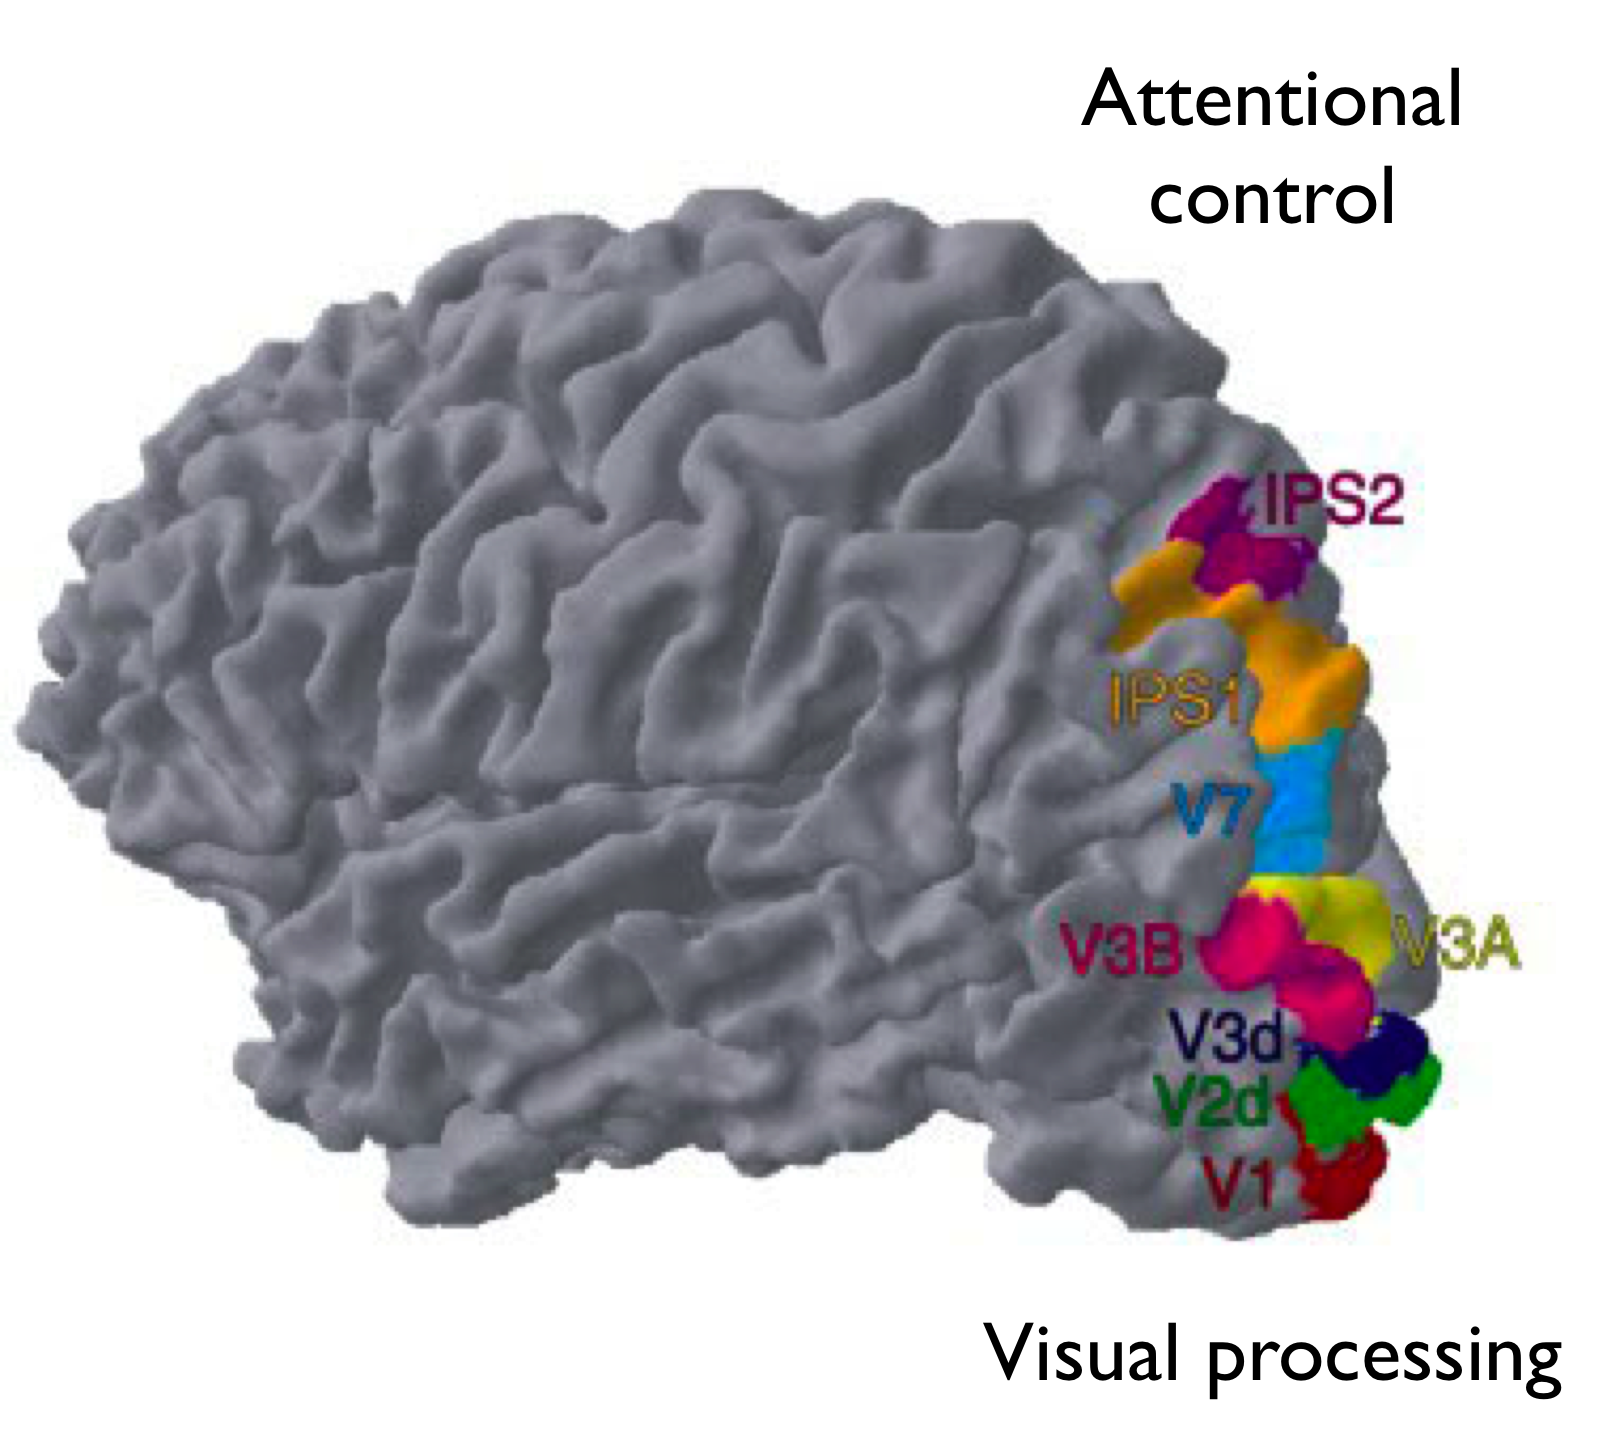
\includegraphics[height=5.7cm]{figures/lauritzen1}
\\
\hfill 
Lauritzen et al. (2009)
\end{frame}

\begin{frame}
\frametitle{Covert attention task}
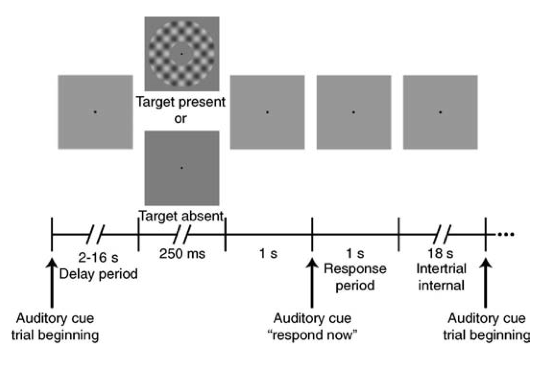
\includegraphics[height=5.7cm]{figures/lauritzen2}
\\
\hfill 
Lauritzen et al. (2009)
\end{frame}

\begin{frame}
\frametitle{Hemodynamic delays}
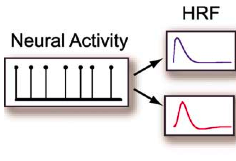
\includegraphics[height=2.7cm]{figures/hemo}
\end{frame}

\begin{frame}
\frametitle{Hemodynamic delays}
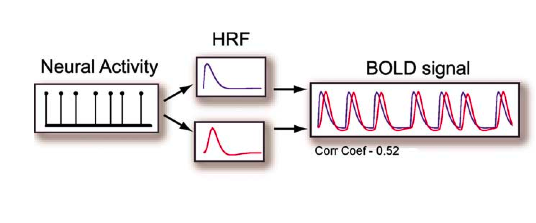
\includegraphics[height=3.7cm]{figures/tseries_w_hemo}
\end{frame}

\begin{frame}
\frametitle{Coherency}
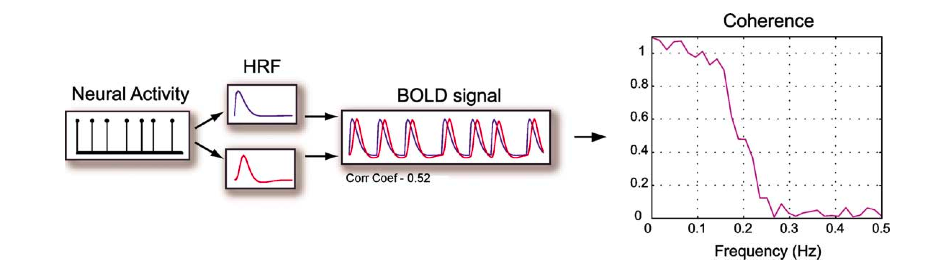
\includegraphics[height=2.7cm]{figures/tseries_w_hemo_w_coh}
\\
\hfill
Sun et al. (2004,2005)
\end{frame}

\begin{frame}
\frametitle{Coherency}
A spectral analog of correlation
\end{frame}

\begin{frame}
\frametitle{Coherency}
$C_{xy}(\omega) = \frac{f_{xy}(\omega)}{\sqrt{f_{xx}(\omega)f_{yy}(\omega)}}$
\pause
\\
\vfill
Where, $f_{xy}$ is the cross-spectral density and 
\\
$f_{xx}$ is the PSD of $x$
\end{frame}

\begin{frame}
\frametitle{Coherency}
Coherency is complex-valued:
\\
\vfill
\pause
Coherence: $Coh_{xy} (\omega) = abs(C_{xy}(\omega)) = $
\pause
$\frac{|f_{xy}(\omega)|^2}{f_{xx}(\omega)f_{yy}(\omega)}$
\pause 
\\
\vfill
Ranges from $0$ to $1$
\end{frame}


\begin{frame}
\frametitle{Baseline coherence}
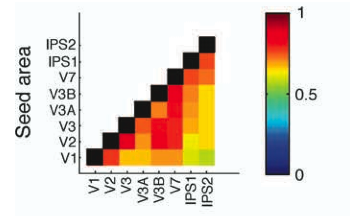
\includegraphics[height=2.7cm]{figures/lauritzen3}
\\
\hfill 
Lauritzen et al. (2009)
\end{frame}

\begin{frame}
\frametitle{Attention coherence}
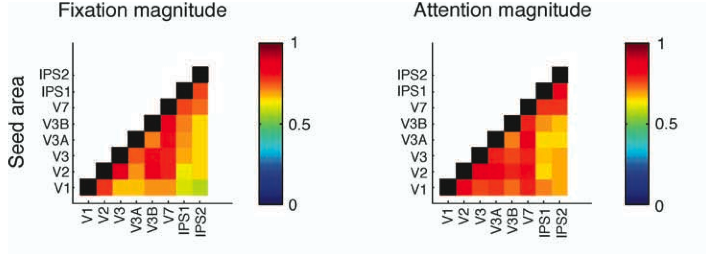
\includegraphics[height=2.7cm]{figures/lauritzen4}
\\
\hfill 
Lauritzen et al. (2009)
\end{frame}

\begin{frame}
\frametitle{Difference in coherence}
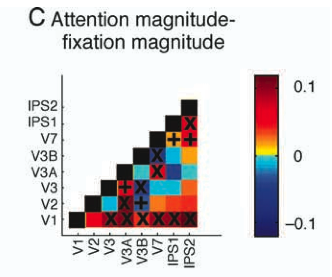
\includegraphics[height=5.7cm]{figures/lauritzen5}
\\
\hfill 
Lauritzen et al. (2009)
\end{frame}

\begin{frame}
\frametitle{Coherency}
Coherency is complex-valued:
\\
\vfill
Coherence: $Coh_{xy} (\omega) = abs(C_{xy}(\omega)) = $
$\frac{|f_{xy}(\omega)|^2}{f_{xx}(\omega)f_{yy}(\omega)}$
\\
\pause
\vfill
Phase: $\phi(\omega)= angle(C_{xy}) =
tan^{-1}\frac{\Im(f_{xy}(\omega))}{\Re(f_{xy}(\omega))}$
\vfill
\pause
Ranges from $-\pi$ to $\pi$
\end{frame}

\begin{frame}
\frametitle{Time delay}
The time-delay between two time-series can be calculated from the phase delay 
\\ 
\pause
\vspace{1cm}
$\Delta t (\omega) = \frac{\phi(\omega)}{2 \pi \omega}$
\end{frame}

\begin{frame}
\frametitle{Time delay}
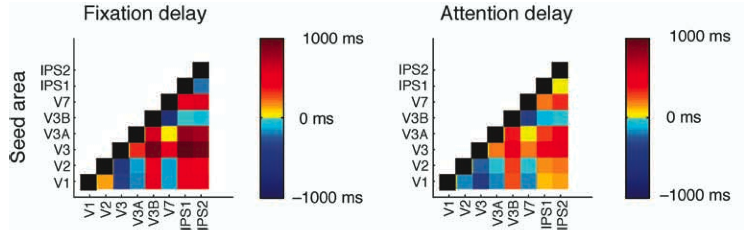
\includegraphics[height=2.7cm]{figures/lauritzen6}
\\
\hfill 
Lauritzen et al. (2009)
\end{frame}

\begin{frame}
\frametitle{Delay difference}
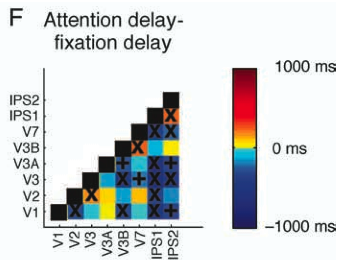
\includegraphics[height=5.7cm]{figures/lauritzen7}
\\
\hfill 
Lauritzen et al. (2009)
\end{frame}

\begin{frame}
\frametitle{Task-related network changes:}
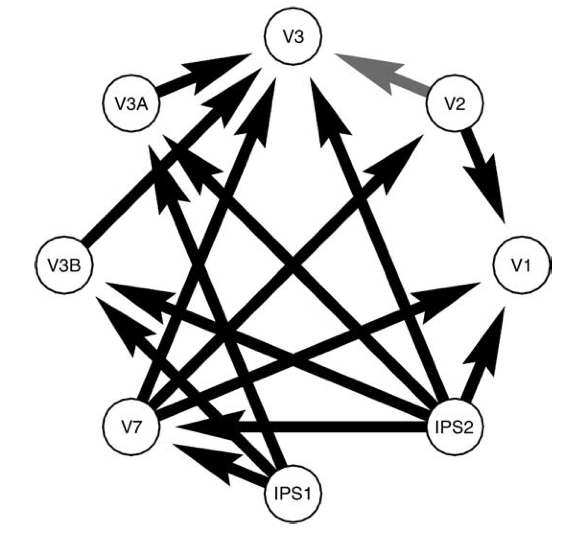
\includegraphics[height=5.7cm]{figures/lauritzen8}
\\
\hfill 
Lauritzen et al. (2009)
\end{frame}

\begin{frame}
\frametitle{\tt{Nitime}}
\begin{itemize}
\pause
\item
Software library for the analysis of time-series from neuroscience data
\pause
\item
Written in Python
\pause
\item 
Free and open source
\pause
\item
Part of the \tt{NIPY} \sc{project}
\pause
\item
\tt{http://nipy.org/nitime}
\end{itemize}
\end{frame}

\begin{frame}
\frametitle{Why Python?}
\begin{itemize}
\pause
\item
A full-fledged programming language
\pause
\item
OO is built in 
\pause
\item
Powerful testing frameworks (sphinx)
\pause
\item
Documentation framework (nose) 
\pause
\item
Libraries for scientific computing (numpy, scipy)
\pause
\item
Libraries for visualization (2D: matplotlib, 3D: mayavi).
\pause
\item 
For more details see: 
\end{itemize}
\end{frame}

\begin{frame}
\frametitle{\tt{nitime} components:}
\begin{itemize}
\begin{tt}
\pause
\item
nitime.timeseries
\pause
\item
nitime.viz
\pause
\item
nitime.algorithms
\pause
\item
nitime.analysis
\pause 
\item
nitime.utils
\end{tt}
\end{itemize}
\end{frame}

\begin{frame}[fragile]
\frametitle{TimeSeries example:}
\pause
\begin{lstlisting}
>>> import nitime.timeseries as ts 
>>> t1 = ts.TimeSeries(data=[1,2,3,4],
                       sampling_interval=1.5,
                       time_unit='s')
\end{lstlisting}

\pause
\begin{lstlisting}
>>> t1.time
UniformTime([ 0. ,  1.5,  3. ,  4.5], 
                       time_unit='s')
\end{lstlisting}

\pause
\begin{lstlisting}
>>> t1.sampling_rate
0.666666666667 Hz
\end{lstlisting}

\end{frame}

\begin{frame}[fragile]
\frametitle{Vizualization}
\pause
\begin{lstlisting}
>>> import nitime.viz as viz
>>> viz.plot_tseries(t1)
\end{lstlisting}
\end{frame}

\begin{frame}
\frametitle{Vizualization}
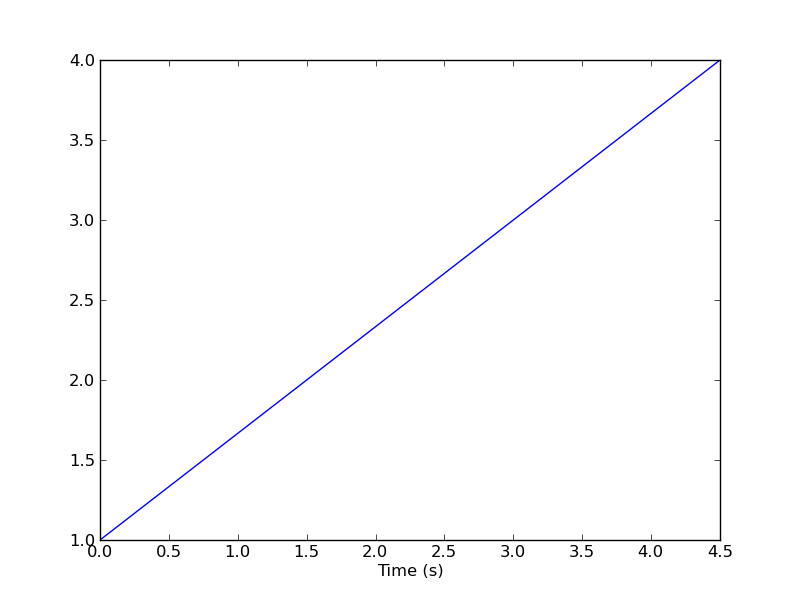
\includegraphics[height=5.7cm]{figures/simple_viz}
\end{frame}

\begin{frame}[fragile]
\frametitle{Vizualization}
\begin{lstlisting}
>>> t2 = ts.TimeSeries(data=np.sin(
                       np.linspace(0,2*np.pi)),
                       sampling_interval=0.1,
                       t0=-2, 
                       time_unit='ms')
>>> viz.plot_tseries(t2)
\end{lstlisting}
\end{frame}

\begin{frame}
\frametitle{Vizualization}
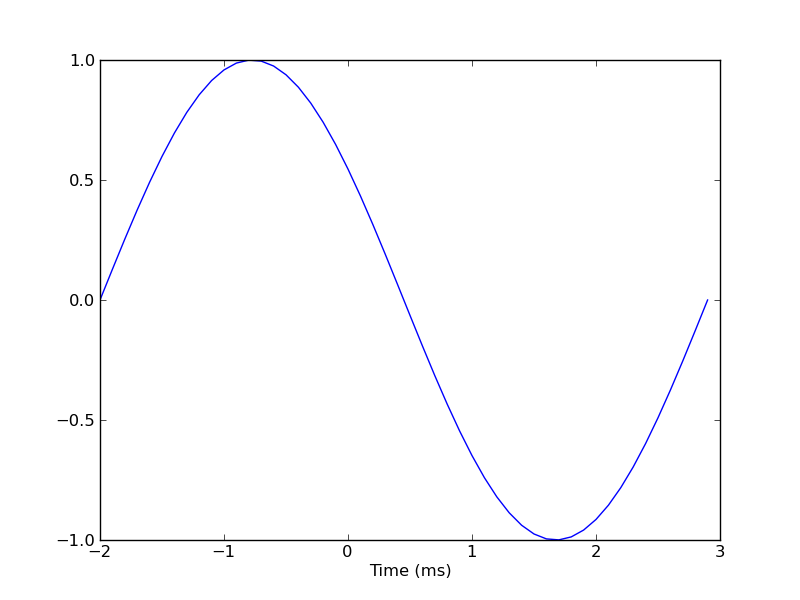
\includegraphics[height=5.7cm]{figures/simple_viz2}
\end{frame}


\begin{frame}
\frametitle{\tt{nitime.algorithms}}
\begin{itemize}
\pause
\item
Provides a functional interface based on numpy arrays
\begin{tt}
\pause
\item
coherence
\pause
\item
event-related
\pause
\item
filter
\pause
\item
spectral
\item
\pause
autoregressive
\end{tt}
\pause
\item
These implementations accept arrays as their inputs, not \tt{TimeSeries}!
\end{itemize}
\end{frame}

\begin{frame}[fragile]
\frametitle{Example: univariate analysis}
\pause
\begin{lstlisting}
>>> noise = 0.5
>>> t = np.linspace(0,8*pi,1024) 

>>> x =  (np.sin(5*t) + np.sin(1.33*t) +  
     noise*np.random.randn(t.shape[-1]))

>>> y =  (np.sin(5*t + pi/4) + 
          np.sin(1.33*t-pi/2) +
     noise*np.random.randn(t.shape[-1]))
\end{lstlisting}

\pause
\begin{lstlisting}
>>> t3 = ts.TimeSeries(np.vstack([x,y]),
                sampling_rate=np.pi)
\end{lstlisting}

\pause
\begin{lstlisting}
>>> viz.plot_tseries(t3)
\end{lstlisting}
\end{frame}

\begin{frame}
\frametitle{Time-series}
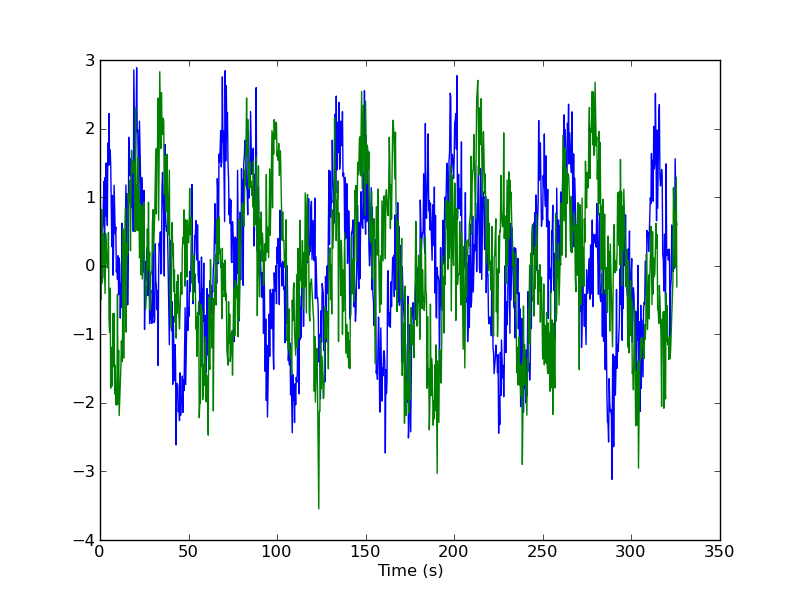
\includegraphics[height=5.7cm]{figures/outa_phase_tseries}
\end{frame}

\begin{frame}[fragile]
\frametitle{Univariate analysis: spectral analysis }
\begin{lstlisting}
>>> import nitime.algorithms as alg
\end{lstlisting}
\pause
\begin{lstlisting}
>>> method = {'this_method':'welch',
              'Fs':np.pi,
              'NFFT':256}
\end{lstlisting}
\pause
\begin{lstlisting}
>>> f, c = alg.get_spectra(t3.data,method=method)
\end{lstlisting}
\pause
\begin{lstlisting}
>>> plt.plot(f, c[0,0])
\end{lstlisting}
\end{frame}

\begin{frame}
\frametitle{Univariate analysis: spectral analysis}
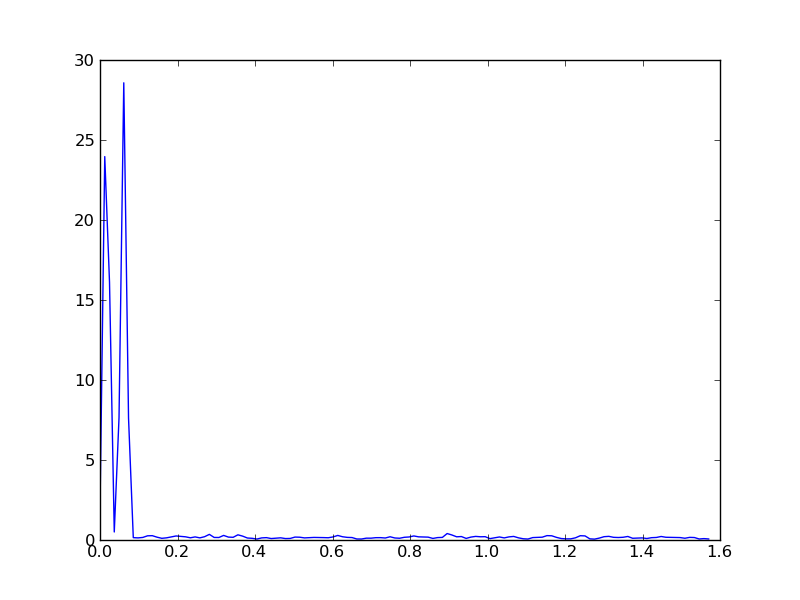
\includegraphics[height=5.7cm]{figures/outa_phase_tseries_single_psd}
\end{frame}

\begin{frame}
\frametitle{\tt{nitime.analysis}}
\begin{itemize}
\pause
\item 
Provides a more stream-lined analysis interface
\pause
\item 
'Knows' about \tt{TimeSeries} \sc{objects and accepts them as inputs}
\pause
\item
\tt{coherence}
\pause
\item
\tt{correlation}
\pause
\item
\tt{event-related}
\pause
\item
\tt{normalization}
\pause
\item
\tt{snr}
\item
\pause
\tt{spectral}
\item
\pause
\tt{Granger 'causality'}
\end{itemize}
\end{frame}

\begin{frame}
\frametitle{Bivariate analysis 1: cross-correlation}
$Rxy(\tau) = \sum_{i=0}^{T}{x(t)y(t+\tau)}$
\end{frame}

\begin{frame}[fragile]
\frametitle{Bivariate analysis 1: cross-correlation}
\pause
\begin{lstlisting}
>>> import nitime.analysis as nta
\end{lstlisting}

\pause
\begin{lstlisting}
>>> XC = nta.CorrelationAnalyzer(t3) 
\end{lstlisting}

\pause
\begin{lstlisting}
>>> viz.plot_xcorr(XC.xcorr_norm,[[0,1]])
\end{lstlisting}
\end{frame}

\begin{frame}
\frametitle{Bivariate analysis 1: cross-correlation}
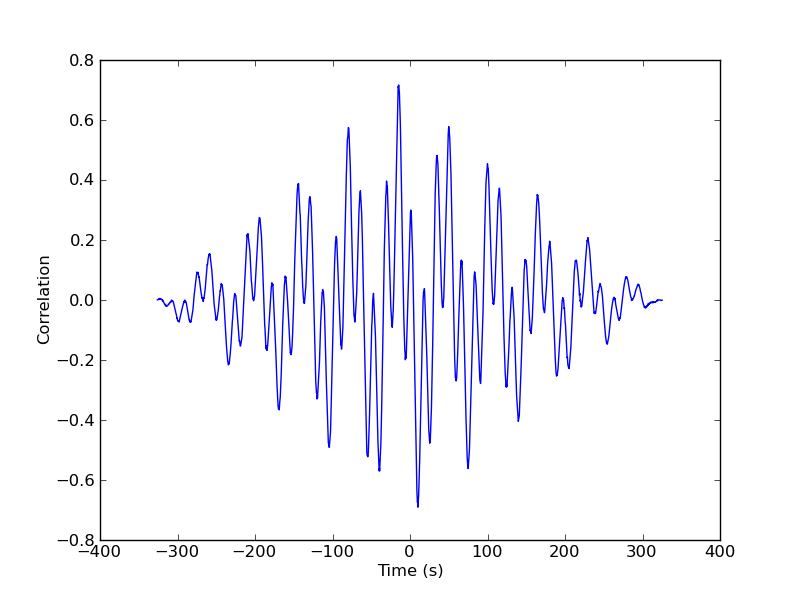
\includegraphics[height=5.7cm]{figures/outa_phase_xcorr}
\pause 
\\
$r_{xy}=0.25$
\end{frame}

\begin{frame}[fragile]
\frametitle{Bivariate analysis 2: Coherence}
\begin{lstlisting}
>>> plt.plot(C.frequencies, C.coherence[0,1])
\end{lstlisting}
\end{frame}

\begin{frame}
\frametitle{Coherence}
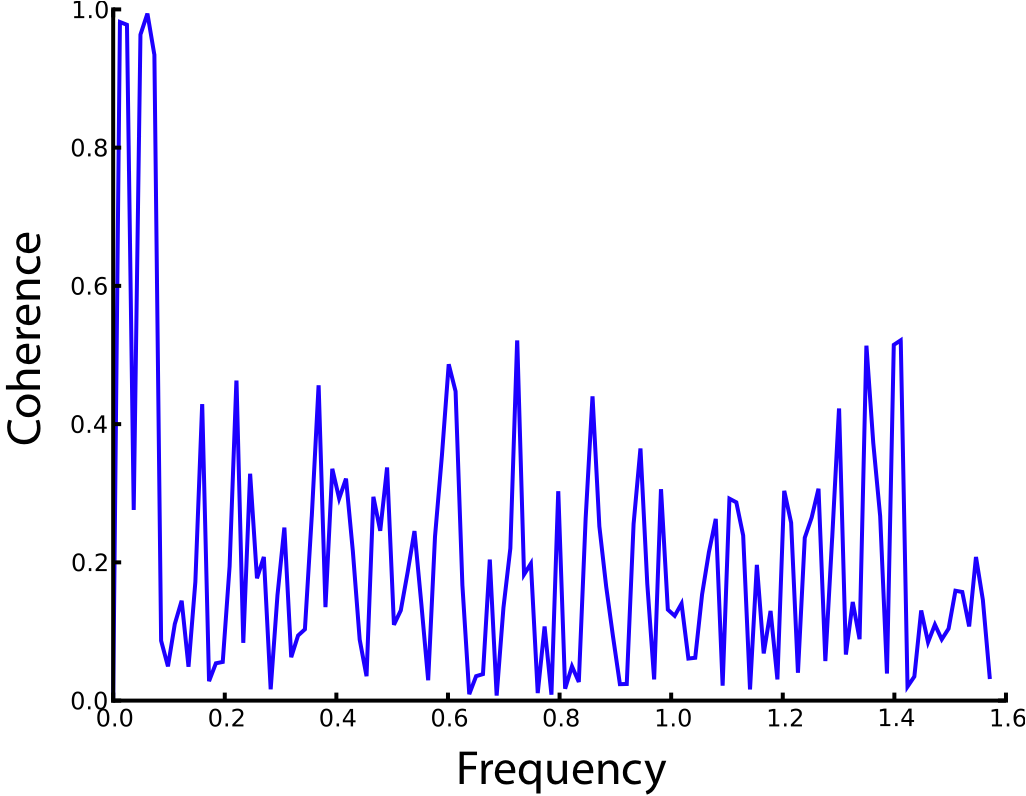
\includegraphics[height=5.7cm]{figures/outa_phase_tseries_coh}
\end{frame}

\begin{frame}[fragile]
\frametitle{Phase}
\begin{lstlisting}
>>> plt.plot(C.frequencies, C.phase[0,1])
\end{lstlisting}
\end{frame}

\begin{frame}
\frametitle{Phase}
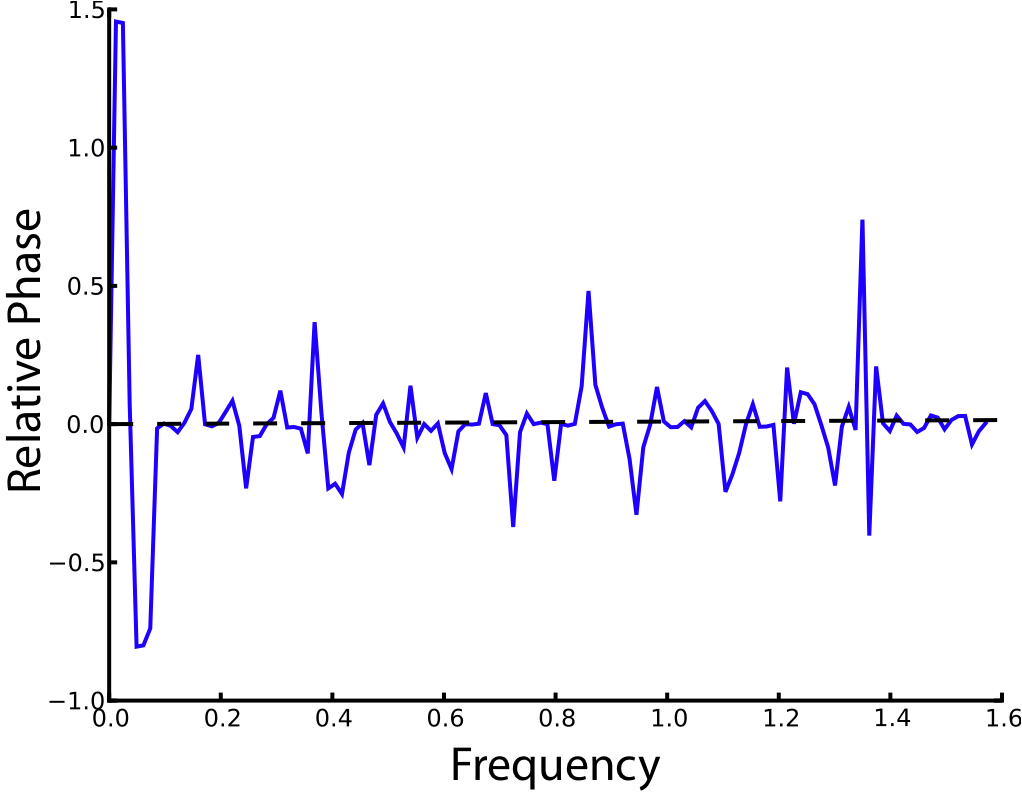
\includegraphics[height=5.7cm]{figures/outa_phase_tseries_ph}
\end{frame}

\begin{frame}[fragile]
\frametitle{Not surprising}
\begin{lstlisting}
>>> noise = 0.5
>>> t = np.linspace(0,8*pi,1024) 

>>> x =  (np.sin(5*t) + np.sin(1.33*t) +  
     noise*np.random.randn(t.shape[-1]))

>>> y =  (np.sin(5*t + pi/4) + 
          np.sin(1.33*t-pi/2) +
     noise*np.random.randn(t.shape[-1]))
\end{lstlisting}
\end{frame}


\begin{frame}
\frametitle{More examples}
http://nipy.org/nitime/examples
\end{frame}

\begin{frame}
\frametitle{Summary: \tt{nitime}}
\begin{itemize}
\pause
\item
\tt{nitime} \sc{provides tools for representing and visualizing time-series and
  derived quantities}
\pause
\item
Implements several univariate and bi-/multi-variate algorithms for time-series
analysis 
\end{itemize}
\end{frame}

\begin{frame}
\frametitle{Integration with mrVista}
http://github.com/arokem/vista\_utils
\end{frame}

\begin{frame}
\frametitle{Thanks!}
\pause
Fernando Perez

Mike Trumpis

Kilian Koepsell

Paul Ivanov

\pause
The NIPY developers

Matthew Brett 

\pause
Neurodebian (Yaroslav and Michael)

\pause
Emi Nomura 

Caterina Gratton 

Ayelet Landau 

Thomas Lauritzen

\pause
Mark D'Esposito 

Michael Silver
\end{frame}


\end{document}
